\documentclass[11pt,oneside]{amsart}
\usepackage{alttpreamble}
% \usepackage{tocloft}
% \renewcommand\cftchapdotsep{\cftdotsep}
\usepackage{fancyhdr}
\pagestyle{fancy}
\begin{document}
\lhead{Fredrick Mooers}
\chead{Journal}
\rhead{\rightmark \today}
\tableofcontents
\newpage

\section{Jun 22}
\subsection{Flooding} This weekend we started work on the ``flooding'' algorithm which works and is great at detecting these super contractible Reeb chords. We could only prove that the algorithm terminates for knots in plat position (our algorithm works equally well for the front and Lagrangian projections). One plan of attack we tried was to see if we could work inductively, assuming we already have a knot isotopic to a knot who's flooding algorithm terminates, we can conclude that every knot's algorithm terminates since every knot can be put in plat position. Planar isotopy doesn't change the structure of our algorithm, but Reidemiester moves are really hard to figure out and we'll need to explore further. I tried RII, by looking at how the inequalities change by adding two new crossings and it's not obvious: I need to look at how the discs change and what disks are born. There are four cases I would need to consider depending on the cusp direction and strand slope, which makes me less excited to think about it.

The current terminology for the algorithm corresponds to flooding the enclosed regions of the knot diagram. The only time our algorithm wouldn't terminate (the stopping criterion is when no equations left can be eliminated) is if all of the remaining Reeb heights have negative coefficients in at least one of the remaining height inequalities. The corresponding enclosed areas attached to these remaining inequalities are called islands, which is pretty cute terminology.

\subsubsection{Stabilization} Certainly the LCH of a stabilized knot is trivial if we argue contractibility of the added crossing (loop).\footnote{I think the stabilization of a knot in plat position has no islands, and it wouldn't be terribly difficult to prove. Perhaps the new crossing is super contractible, but I can't say that with confidence. There's only so many things I can sit down and do.} The triviality of the persistent LCH of a stabilized knot depends on the height assigned to this new crossing: normally you let it be smaller than every other crossing so no possible differential can exist, but having a height be made arbitrarily small isn't necessary condition for a differential to not exist, so there is wiggle room to assign a different height to this crossing. In the future it would be interesting to see how are algorithm works with stabilized knots.

\subsection{Cobordisms and $A_\infty$} Since the start of the week, I've become a little nervous about how much we're doing is original. The Sabloff and Traynor paper gives a filtration and shows that a cobordism $L$ induces a filtered map $\Phi_\ast^{L,I}$ of the Chekanov-Eliashberg DGAs (see proposition 4.2 in \href{https://arxiv.org/pdf/2101.03760.pdf}{this} paper). This shows that isotopies preserve Reeb height since the DGA maps induced by the corresponding cobordisms are just the stable tame maps. The papers are dense, so I would need to think about it more before I get ahead of myself. If I'm just looking at the Sabloff and Traynor paper, we are doing something different with our filtration. In the end, when we do contact cohomology, we'll have to pick a filtration corresponding to the kernel of $i^\ast:\hom(\AlgL, \Z_2)\rightarrow \hom(\AlgL^r, \Z_2)$ where $i:F^r \AlgL^r\rightarrow \AlgL$ is the inclusion.


\subsection{Filtered Knot / Manifold} 

Our flooding algorithm gives us a way to filter the knot diagram (in either projection) by just removing the enclosed areas corresponding to the removed inequalities in the algorithm up to a certain time step. It's not the diagram of any knot because you might have what were once crossings, now becoming a T-shaped intersection. It could be possible to resolve these singularities in some way to get a knot diagram with DGA closely related to the original knot DGA at a certain time step, which was what Austin suggested in one of our lectures.

Another related idea, is to look at the zero resolution cobordisms. It seems like our algorithm should respect this kind of resolution, which corresponds to running our algorithm on the same set of inequalities but with the contractible Reeb chord height set to zero.

\section{Jun 27}

\subsection{Filtered Knot / Manifold pt. 2} My current intuition for the flooding algorithm is that each area patch is a disk in the diagram, and you remove these area patches at each time step in the flooding algorithm. This interpretation is nice, because extras can be read off easily (in plat position) by the fact that at some point in the algorithm there will be empty space to the left and right of the crossing (empty in the sense there is no area patch with positive corners touching that crossing) corresponding to the fact every equation the crossing appears in. The only real obstruction to this outside of plat, that I can think of right now, is if the crossing corresponds to an interior loop.

\subsection{Contractibles in Plat} Our algorithm enumerates contractibles in plat position. In retrospect it's clear what the contractibles are in that case, but it's also important to note that they fall into 3 categories there, that may be relevant to our study of persistent LCH. One next step in this line of enumerating contractibles is to see how our algorithm is changed by reidemeister moves, which is already highly non-obvious, but may lead to interesting questions.

\subsection{Reidemister Moves} To figure out stuff with persistent stable tame isomorpisms we figured we could look at both examples and try to prove things from just the crossing. We first thought about doing it in the Lagrangian projection, but then realized we used L2 and got an invalid Legendrian knot projection (something went wrong with the differential). We're probably going have to look through Chekanov's original paper to do this in Lagrangian projection. The Front projection Reidemiester moves are slightly more clear, F1 leads to a single stabilization composed with a tame isomorphism and the effect on persistent homology is interesting, creating a finite barcode and then reverting back to the original diagram. There are two cases to F2: left cusp v. right cusp move. The left cusp move is really the same as R2 in the Lagrandian projection, which means single stabilization plus tame isomorphism. Persistent homology in this case is affected similarly as R1 where the barcode is different for a certain time period until it reverts back to the original barcode when one of the new crossings is killed. F3=R3 is just tame isomorphism, and it's effect at the intersection is clear, but away from the intersection is a little less obvious, and we'll have to overall explore tame isomorphisms much more.

\section{My Journal Slacking Jun 27 - Jul 6}

\subsection{Contractibles in Plat False} My proof about classifying knots in plat was wrong because having an area loop inequality of the form $h_i + h_j - (\cdots)>0$ doesn't necessarily mean that either $a_i$ or $a_j$ is contractible as one can have a non-zero differential as seen in the legendrian knot given by the braid closure of $\{4, 3, 2, 3, 2, 4\}$ where $\d a_8 = 1+a_5$ and we have area loop inequality $h_8+h_4-h_5-h_6>0$.

\subsection{The $H$-contractible saga: Research is Hard} The term $H$-contractible has gone through many stages and is still going through many stages.

\subsubsection{\textsc{Pain}: The first coming of trouble} At first to show that the number of non-$H$-contractibles is invariant under isotopy, we looked at the different Reidemeister moves in the front projection, and getting pretty far only with problems with Reidemeister move 2. The problem was we didn't carefully check the height changes assuming the same heights could be used and they can only under certain conditions highlighted in Kalman's paper (like small area of triangle for triple point move).

This was quite problematic as our definition of being not $H$-contractible meant that you had to be able to bound below the length of the bar for \textit{any} height assignment and it is now completely non-obvious if such a thing can be done after preforming a Reidemeister move. In essence, this just means that the space of valid height assignments before is not the same as the space of valid height assignments after preforming the Reidemeister move. In essence, we now need to either restrict the possible isotopies we can preform or find alternative criterion for $H$-contractibility.

\begin{figure}[htbp]
  \label{fig:Figure8}
  \centering
  \includesvg{figureeight.svg}
  \caption{Figure eight knot with red region area $a_4-a_3$. It's also worth noting here that the bar corresponding to generator $a_5$ (or $a_6$) isn't $H$-contractible since $a_4$ isn't contractible so $h_2$ can't be shrunk down to $h_5$ as in the definition of $H$-contractible.}
\end{figure}

We tried the latter first see if $H$-contractibility can be described by the height changes given by disks corresponding to words in the differential. This proved unsuccessful since we found a height inequality $a_4>a_3$ in Figure \ref{fig:Figure8} above. Now coincidentally we have $|a_4|-|a_3|=(2-3)+(2-1)=0$ so that this height inequality doesn't effect any deaths in the barcode of the figure eight knot LCH. Interesting to note that non-$H$-contractibles, if they depend on inequalities not coming from the differential alone, are probably not isotopy invariant by the fact that the Reidemeister move preformed in the figure above now makes it so that $h_4$ isn't necessarily bigger that $h_3$.


\section{Jul 7}

Cool inequality:
\begin{theorem}
    Let $\L_-$ and $\L_+$ be Legendrian isotopic related by a planar isotopy in $\R^2_{xy}$. Let $B_\pm$ correspond to a finite bar in $\L_\pm$ generated by $\sum_{i}a_i^{\pm}$ and killed by $\sum_{j}b_j^{\pm}$. Then $\max_j(h(b_j^+)-h(b_j^-))-\max_i(h(a_i^+)-h(a_i^-))\leq \ell(B_+)-\ell(B_-)$.
\end{theorem}
\begin{proof}
    We know that the length $\ell(B_\pm)=\max_j(h(b_j^\pm))-\max_i(h(a_i^\pm))$. From the inequality $\max_i(c_i-d_i)\leq \max_i(c_i)-\max_i(d_i)$, we see that $\max_i(h(a_i^+)-h(a_i^-))\leq \max_i(h(a_i^+))-\max_i(h(a_i^-))$. But then we see that
    \begin{align*}
        \max_j(h(b_j^+)-h(b_j^-))-\max_i(h(a_i^+)-h(a_i^-))&\leq \max_j(h(b_j^+))-\max_j(h(b_j^-))+\max_i(h(a_i^-))-\max_i(h(a_i^+))\\&=(\max_j(h(b_j^+))-\max_i(h(a_i^+)))+(\max_j(h(b_j^-))-\max_i(h(a_i^-)))\\&=\ell(B_+)-\ell(B_-).\qedhere
    \end{align*}
\end{proof}

{\color{red}\textsc{It has come to my attention that the above is wrong because when doing the $\Delta h(b)$'s I used the reverse of the inequality that was actually correct.}}

\section{Jul 10}
\subsection{Islands exist and the flooding algorithm fails}
We can do some Lagrangian Reidemeister moves on the trefoil to make our algorithm fail. See Figure \ref{fig:failure}:
\begin{figure}
    \centering
    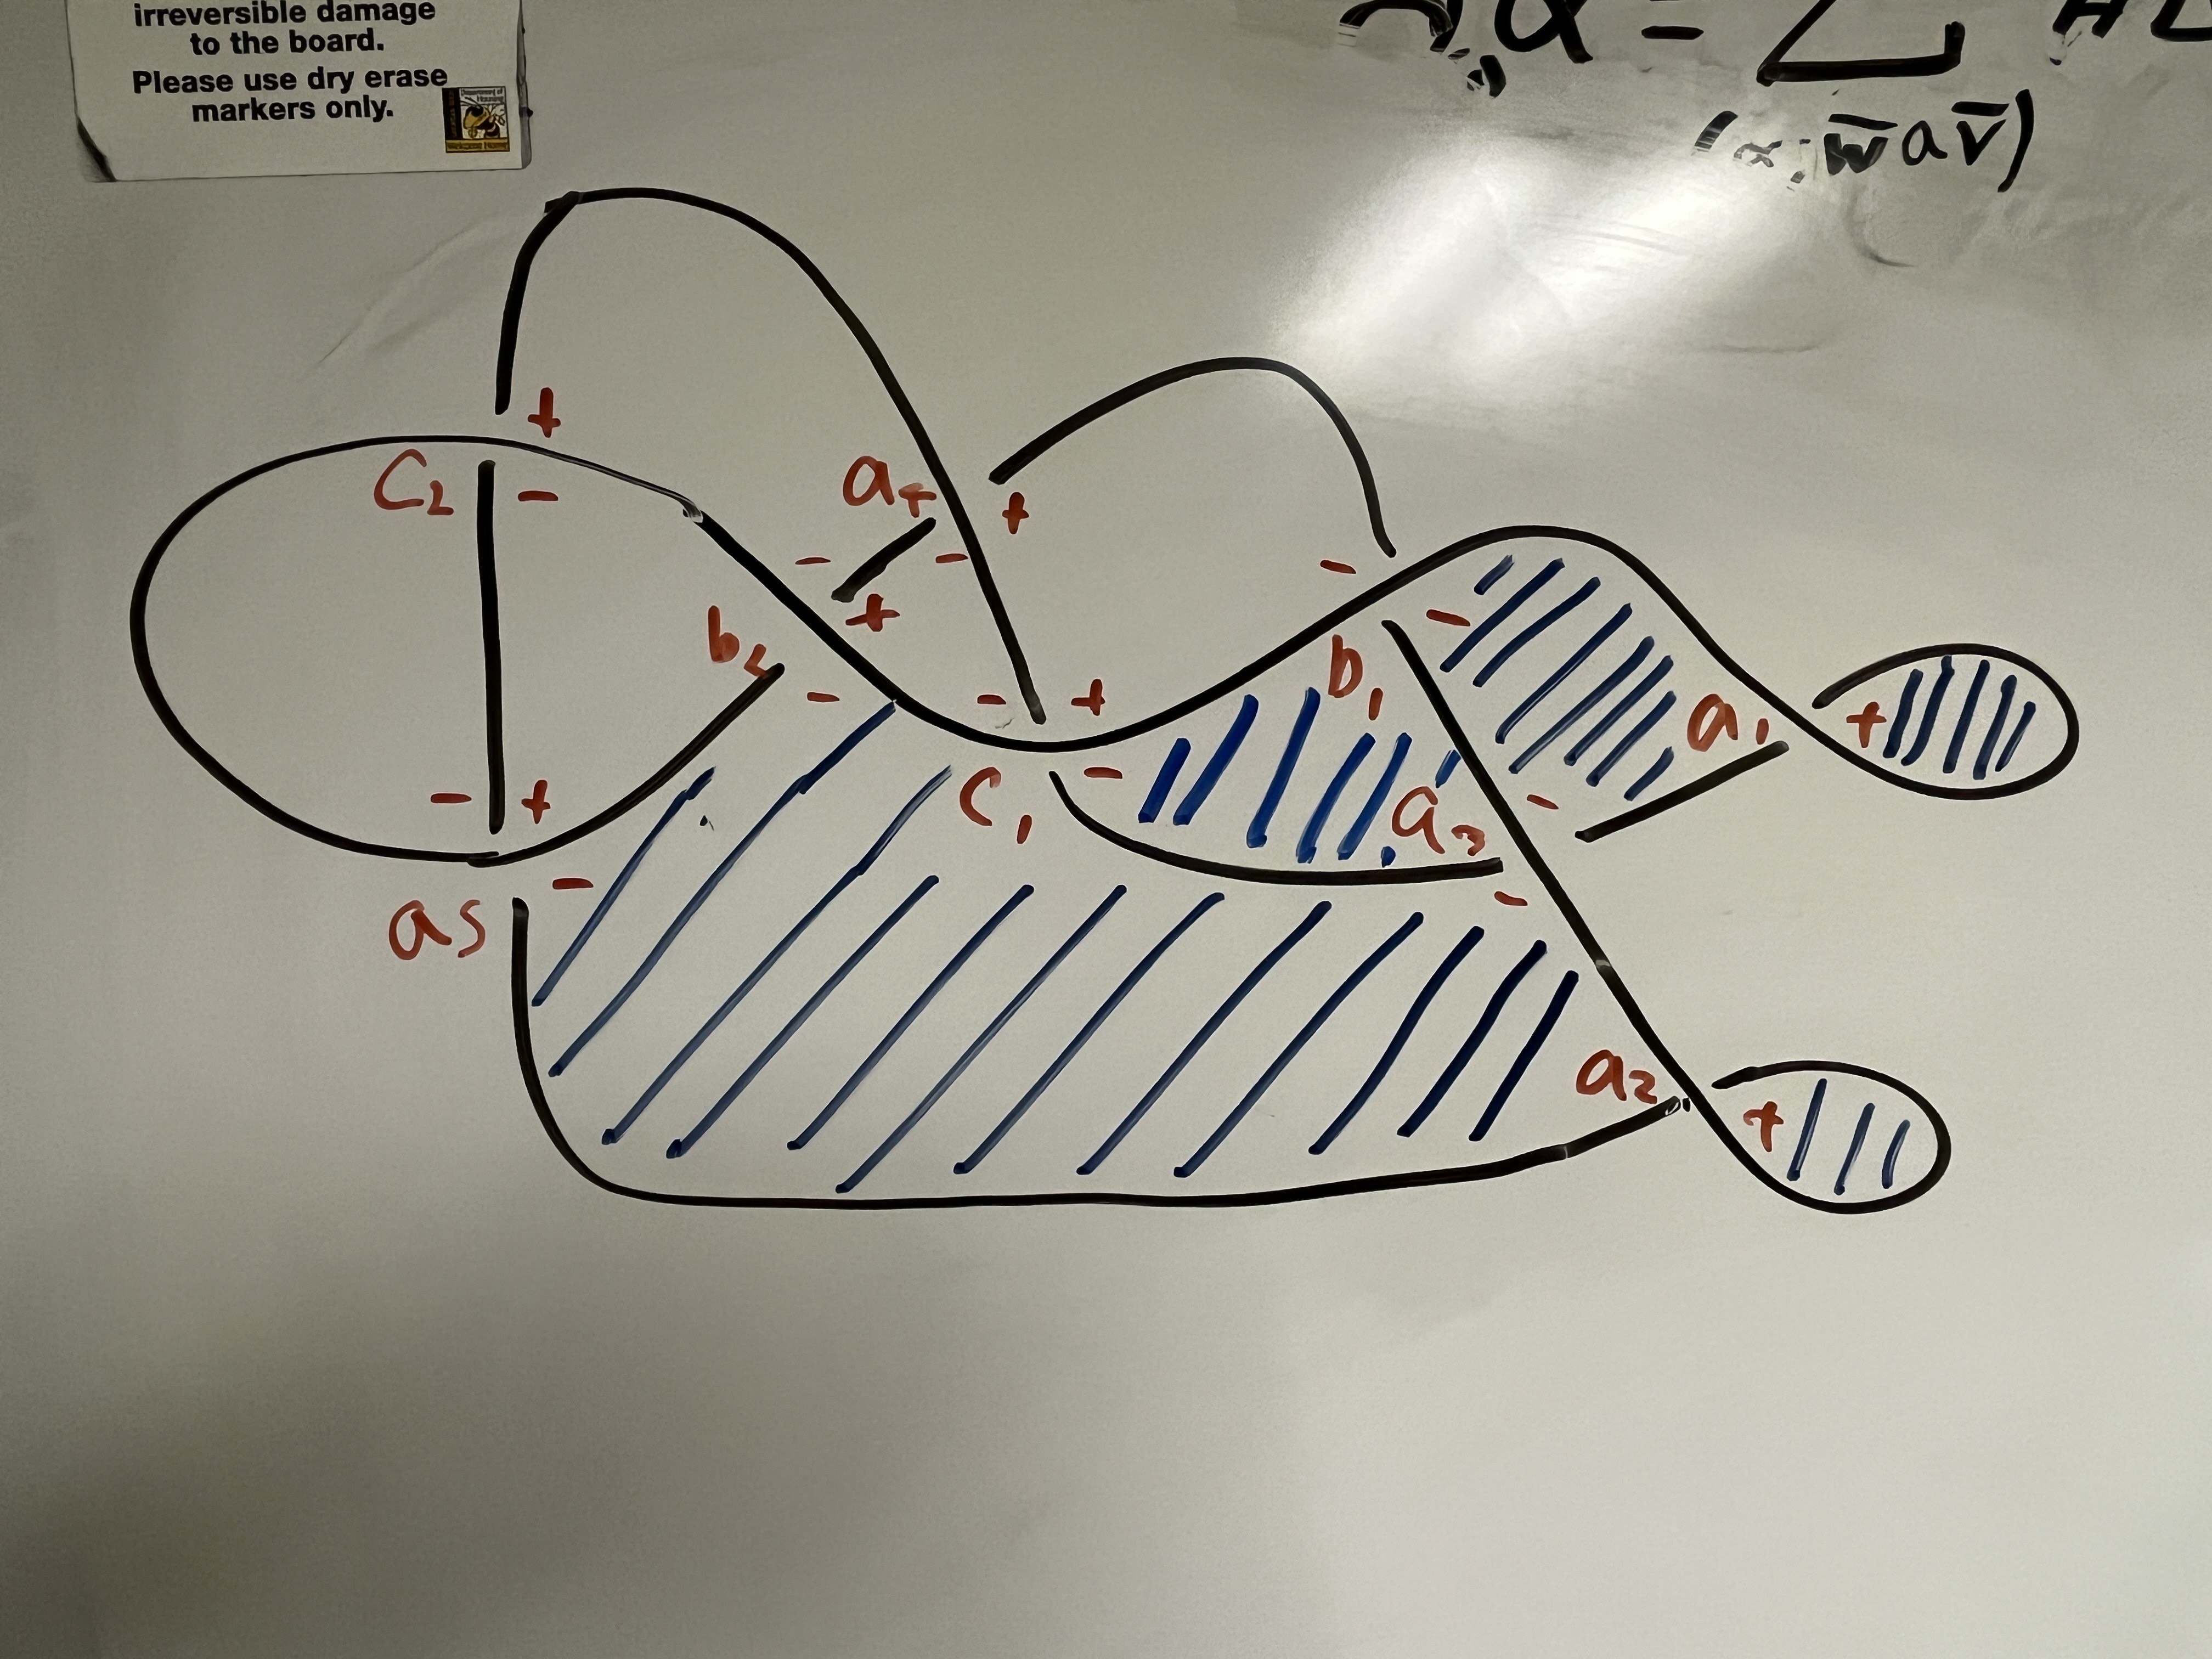
\includegraphics[width=\linewidth]{Journals/IMG_2741.jpg}
    \caption{Flooding algorithm on knot isotopic to standard legendrian trefoil (the island trefoil). Note that the flooding algorithm stops after flooding the disk with $a_3$ in it, because the rest of the heights that appear positive in the remaining inequalities appear negative in another inequality. }
    \label{fig:failure}
\end{figure}
We've tried many fixes, none of them succeeding to give something satisfying.
\subsection{$m_2$ pipe dream}
For all $\epsilon>0$, does there exists a planar isotopy such that the barcode corresponding to the $m_2$ product and the barcode corresponding to the tensor product agree by some $2\delta$-interweaving for some $\delta$ depending on $\epsilon$? This really just means making the tensor product of bars close to the bar corresponding to the $m_2$ product. Maybe just need a planar isotopy that makes the two diagrams somewhat close.

In some sense, we can just do all of this in plat position and that would be a pretty good result by itself. Potentially we could also look at how Reidemeister moves affect this but it's not something I'm even sure we have time to do.

\section{Jul 11}

I think the main antagonist of this project so far was the fact that the geometry of legendrian knots and the \textit{linearized} contact homology don't relate in a very nice way. It makes proving things very difficult, made worse by the fact that the geometry of legendrian knots doesn't feel very rigid at all. Usually geometry forces the algebra to behave in a very predictable way, but every single idea we've had has been destroyed by translating geometry to liearization and the fact that anything geometric we've come up with can be easily destroyed by Reidemeister moves.

For example, I was trying to work out when the equality $\max(b-c,d-e)=\max(b,d)-\max(c,e)$ and in general with more than two elements, I found that there are so many possibilities from mathematica that it feels almost impossible to characterize (see Figure \ref{fig:mathematica}).

\begin{figure}
    \centering
    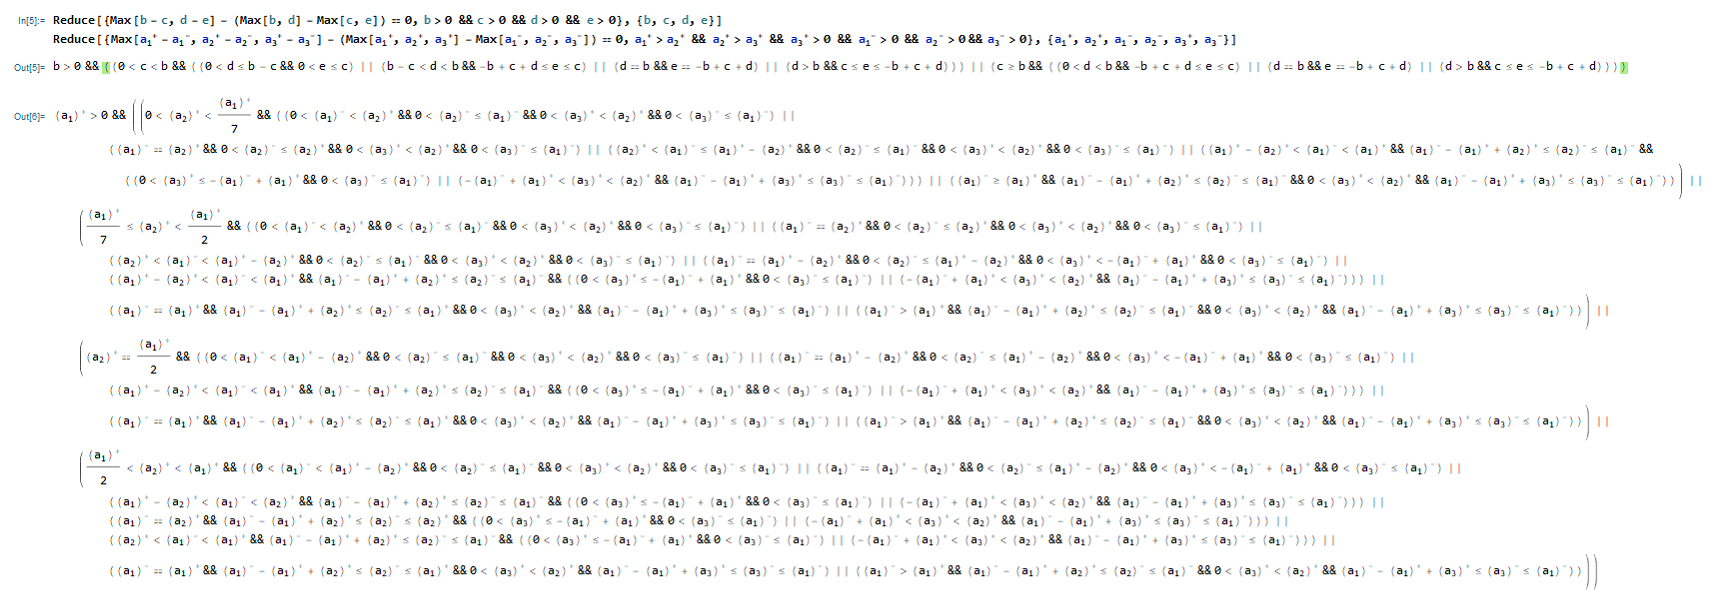
\includegraphics[width=\linewidth]{Journals/mathematicastuff.png}
    \caption{Trying to find solutions to $\max_i(\Delta h(a_i))=\max_i(h(a_i^+))-\max_i(h(a_i^-))$.}
    \label{fig:mathematica}
\end{figure}

I even tried seeing if it was possible to see how the barcode would change if you restrict to planar isotopies that change each individual area by at most $\delta$ and there it was impossible to say anything substantial. The reasoning comes in the form of an example: say we have a finite bar coming from $\partial^\epsilon_{(1)}(b)=\sum_i a_i$. We know that each $a_i$ comes from some word of the form $\mathbf{c}a_i\mathbf{d}$ with $\epsilon(\mathbf{c})=\epsilon(\mathbf{d})=1$. But then all we can say is that $-N_i\delta< \Delta h(b)-\Delta h(\mathbf{c})-
\Delta h(a_i)-\Delta h(\mathbf{d})<N_i\delta$ for some $N_i\in \Z_{\geq 0}$, and so we have no information on the length of the finite bar corresponding to $\sum_i h(a_i)$ because of $h(\mathbf{c})$ and $h(\mathbf{d})$. The augmentation makes arguing about heights near impossible sometimes unless in simple examples like the trefoil.

The only actual thing I proved today was that if the heights change by at most $\delta$, then the length of any bar can change by at most $2\delta$, which is already clear and not very useful.

We finally had something geometric, but nothing came of it because it's too hard! The geometry is not rigid enough. See the other two's journals for the definition of a trapped disk, but it seemed to work so well, only to fail for Reidemeister 3 and essentially fail for Reidemeister 3. We have no reason for this to work, and trying to deal with augmentations is too hard. It's really almost as if we need to just work with the non-linear differential, but we cannot because it's incredibly unruly. At this point we might as well argue things about the characteristic algebra.
\end{document}